\documentclass[11pt]{report}
\usepackage[utf8]{inputenc}
\usepackage[danish]{babel}
\usepackage [T1]{fontenc}
\usepackage[margin=2.5cm]{geometry}
\usepackage[hidelinks]{hyperref}
\usepackage{graphicx}
\graphicspath{{figures/}{Billeder/}}
\usepackage{listings}
\usepackage{color}
\usepackage{adjustbox}
\usepackage{tocloft}
\usepackage{listings}
\usepackage{enumitem}
\usepackage{indentfirst}
\usepackage{caption}
\usepackage{float}

\setlength{\parskip}{12pt}

\definecolor{dkgreen}{rgb}{0,0.6,0}
\definecolor{gray}{rgb}{0.5,0.5,0.5}
\definecolor{mauve}{rgb}{0.58,0,0.82}

\lstset{frame=tb,
  language=Java,
  aboveskip=3mm,
  belowskip=3mm,
  showstringspaces=false,
  columns=flexible,
  basicstyle={\small\ttfamily},
  numbers=none,
  numberstyle=\tiny\color{gray},
  keywordstyle=\color{blue},
  commentstyle=\color{dkgreen},
  stringstyle=\color{mauve},
  breaklines=true,
  breakatwhitespace=true,
  tabsize=3
}



\definecolor{bluekeywords}{rgb}{0.13,0.13,1}
\definecolor{greencomments}{rgb}{0,0.5,0}
\definecolor{turqusnumbers}{rgb}{0.17,0.57,0.69}
\definecolor{redstrings}{rgb}{0.5,0,0}

\lstdefinelanguage{FSharp}
                {morekeywords={let, new, match, with, rec, open, module, namespace, type, of, member, and, for, in, do, begin, end, fun, function, try, mutable, if, then, else},
    keywordstyle=\color{bluekeywords},
    sensitive=false,
    morecomment=[l][\color{greencomments}]{///},
    morecomment=[l][\color{greencomments}]{//},
    morecomment=[s][\color{greencomments}]{{(*}{*)}},
    morestring=[b]",
    stringstyle=\color{redstrings}
    }
\usepackage{amsmath}
\title{Systemudvikling Eksamen}


\author{
  Martin, Frederiksen\\
  \texttt{cph-mf237@cphbusiness.dk}\\
  A klassen
  \and
  Andreas, Vikke\\
  \texttt{cph-av105@cphbusiness.dk}\\
  A klassen
  \and
  Asger, Sørensen\\
  \texttt{cph-as466@cphbusiness.dk}\\
  A klassen
  \and
  William, Huusfeldt\\
  \texttt{cph-wh106@cphbusiness.dk}\\
  A klassen
  \and
  Emil, Bruun\\
  \texttt{cph-eb112@cphbusiness.dk}\\
  A klassen
}

\date{}

\begin{document}
\maketitle

\renewcommand{\cftchapleader}{\cftdotfill{\cftdotsep}}
\tableofcontents
\newpage

\chapter*{1. Indledning}
\addcontentsline{toc}{chapter}{1. Indledning}
Denne rapport vil omhandle udviklingen af en webapplikation, der fungerer som en online webshop af forskellige slags software. Udviklingen af denne webapplikation har været hovedpunktet i dette projekt, med fokus på bestemte praktikker fra de to udviklingsmetoder. De to udviklingsmetoder vi har haft fokus på, er Scrum og Extreme Programming. I løbet af rapporten vil der blive redegjort for, hvilke metoder der er blevet gjort brug af, samt hvilken betydning de har haft for udviklingen af denne webapplikation. Herefter vil vi  diskutere de udfordringer, der er blevet stødt på under udviklingen, hvordan de blev løst og, hvis det ikke kunne lade sig gøre, hvad man potentielt kunne have gjort for at komme videre, med henblik på de udviklingsmetoder der var fokus på.


\chapter*{2. Use Case Diagram}
\addcontentsline{toc}{chapter}{2. Use Case Diagram}
Vi startede vores projekt med at udforme det nedenstående Use Case Diagram for at give alle gruppemedlemmer et indblik i, hvad vi skulle til at udvikle. Use Case Diagrammet gav os mulighed for at lufte idéer til selve systemet, før vi overhovedet begyndte at udvikle noget. Diagrammet fortæller, hvilke aktører der har adgang til de forskellige sektioner, samt hvordan de forskellige sektioner kan hænge sammen.

\begin{center}
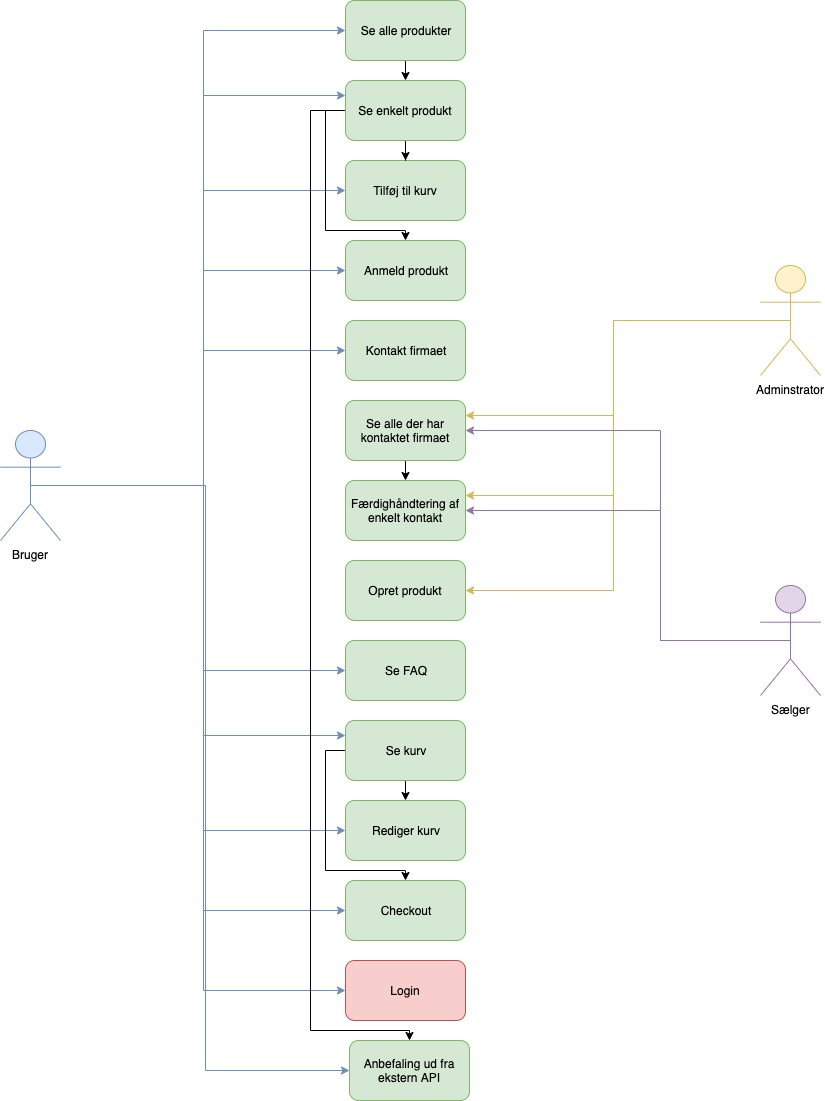
\includegraphics[height=10.5cm, width=15cm]{UseCaseDiagram}
\end{center}

Use Case Diagrammet blev lavet før systemet blev bygget, for at skabe et overblik for gruppen over, hvad for nogle tanker der skulle ligge bag systemudviklingen. Dette gav os et overblik, som gjorde det nemmere at formidle til outsourcer, hvad vi egentlig kunne tænke os rent designmæssigt ud fra den pågældende struktur. Siden da er Use Case Diagrammet blevet opdateret en smule ift., hvad der er blevet lavet og ligeledes farvekoordineret. Der er også blevet lavet en fully dressed Use Case til eksempelvisning (Bilag 1).

\chapter*{3. Outsorcing proces}
\addcontentsline{toc}{chapter}{3. Outsorcing proces}
I dette afsnit vil vi kort redegøre for Outsourcing og processen, for at give indblik i vores oplevelse heraf. Outsourcing betyder at udskille funktioner eller aktiviteter til en underleverandør, som specialiserer sig i emnet, så både højere kvalitet og lavere omkostninger kan opnås. Brugere af outsourcing er ofte virksomheder i lande, hvor omkostningsniveauet er højt, men samtidig gerne vil holde lønomkostninger nede. Dette kan lade sig gøre fordi i lande såsom Indien, skal en ingeniør som er lige så veluddannet i emnet, kun have en tredjedel af den løn en dansk ingeniør ville få.

Det første vi gjorde i outsourcing processen, var at lave en prototype af vores opgave. Vi startede med at udarbejde en analog skitse med papir og blyant, hvor  vi fik tegnet nogle hurtige skitser over alle siderne. Det blev dog hurtigt lavet om til en pænere og mere detaljeret prototype i Adobe XD, som er et prototypeprogram til hjemmesider (Bilag 2). Efter at have udviklet prototypen, skrev vi et jobopslag (Bilag 2). Jobopslaget indeholder en beskrivelse af opgaven, en PDF-fil af prototypen og et prisforslag. Ud over dette blev et Cover Letter også oprettet, som havde til formål at  hjælpe os med at finde den rette til opgaven. Siden Upwork blev brugt til at outsource designet af frontenden, da Upwork er beregnet til større opgaver. Her blev der valgt ikke at outsource React delen af frontenden men kun selve designet. Jobopslaget blev lagt op og kampen om at blive hyret til opgaven begyndte.

\begin{figure}[H]
  \centering
    
\includegraphics[height=8cm, width=15cm]{LandingPage.png}
    \caption*{Landing page - designet af Ahmed Hassan.}
\end{figure}

Vi valgte at have opgaven åben i omtrent 2 dage, for at sikre os at vi modtog et godt tilbud som ikke bare er en automatisk besvarelse fra en computer. Efter de 2 dage havde vi modtaget 12 jobforslag og ud af de 12 jobforslag, valgte vi Ahmed Hassan ud fra hans gode bedømmelser, tidligere arbejde og hans følgebrev. Vi fik også nogle mindre gode ansøgninger såsom Serhii M, der skrev ”Spild ikke din tid på at finde den rigtige kandidat. Jeg er her” og at han kunne klare opgaven på 2 dage og tog halvdelen af den pris vi ville give. Dette syntes vi lød for mærkværdigt.Derfor valgte vi Ahmed, hvorefter korrespondancen (Se bilag 3) gik hurtigt i gang og Ahmed påbegyndte derefter arbejdet til den første milepæl. Vi havde valgt at oprette 3 milepæle i opgaven, som sikrer både os og freelanceren sikkerhed. Freelanceren er dermed sikker på at få de penge han skal, da han allerede efter den første milepæl kan annullere opgaven, hvis betalingen ikke kommer ind. Desuden er også sikret at få leveret den del af opgaven, han har lavet indtil den fastlagte milepæl. Arbejdet med Ahmed gik forrygende, dog var der nogle steder, hvor vi gerne ville have det lidt anderledes, men efter at have fortalt ham det gik der ikke mange minutter, før det var ordnet. Vi kunne have valgt at ordne disse ting selv, men da vi allerede havde Ahmed på opgaven, gjorde det hele processen nemmere ved at få ham til det.

\begin{figure}[H]
  \centering
    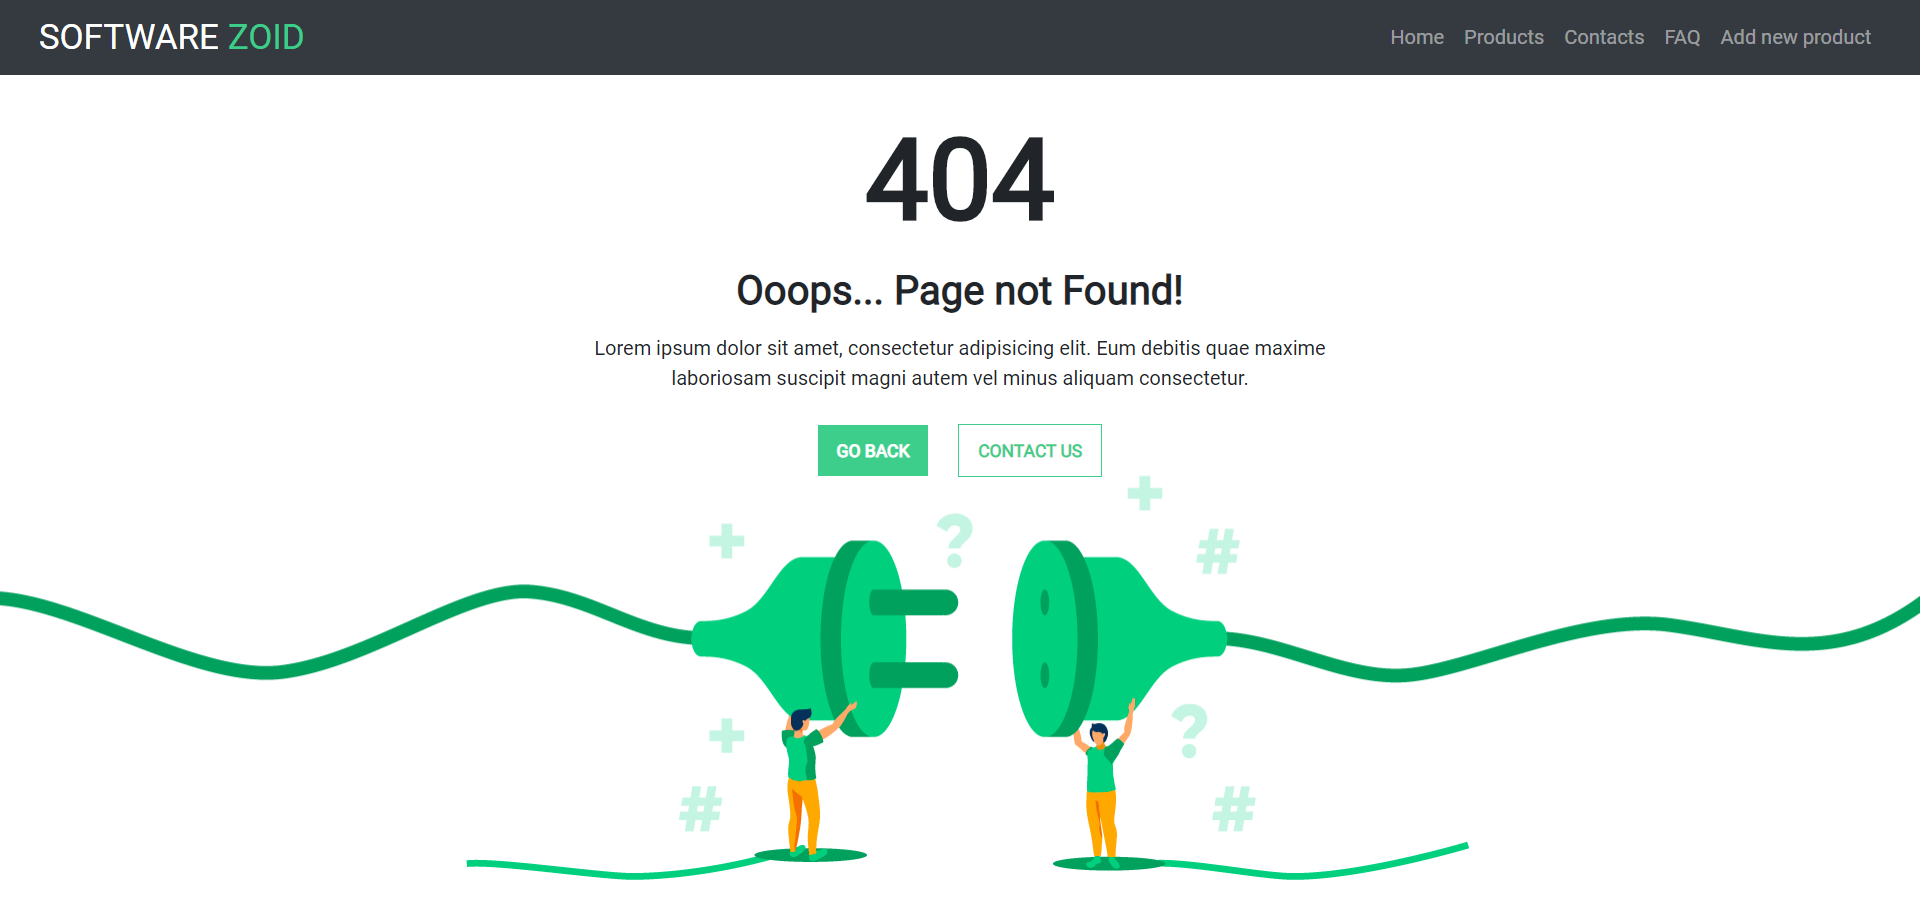
\includegraphics[height=7.5cm, width=15cm]{404Page.png}
    \caption*{404 page - designet af Mizanur.}
\end{figure}

Efter de erfaringer vi havde gjort os med Upwork, ville vi i gruppen forsøge os med en anden outsourcing platform. Her faldt valget på Fiverr grundet dens simple og hurtige måde at arbejde med outsourcing. Et ekstra plus ved Fiverr er, at man på forhånd kender deadlinen for produktet, hvilket havde en stor betydning, da valget blev truffet midt i udviklingsperioden. Tanken bag var også at tvinge en ‘dårlig’ oplevelse. Et eksempel kan være at man får et ubrugeligt produkt tilbage (forkert filformat, el. at det er irrelevant i forhold til projektet, etc.)  
På Fiverr vælger man en outsourcer ud fra hans foruddefinerede opgave. Herefter hyrer man ham og sender en prototype, men ikke noget jobopslag da man allerede har fundet outsourceren. Vi valgte ikke at lave en prototype og skrive meget lidt information for at se, hvad en freelancer med mangelfuld information og ingen prototype kunne komme op med. Korrespondancen (Se bilag 4 og 5) var enkelt og kort og ligesom på Upwork gik dette forrygende. Vi fik udleveret opgaverne til tiden og opgaverne blev lavet tilfredsstillende. Man kunne godt se at stilen ændrede sig fra freelancer til freelancer, men de gjorde alle et virkelig godt job. Forsøget med at få en dårlig oplevelse med outsourcing mislykkede dermed.

\begin{figure}[H]
  \centering
    \includegraphics[height=4cm, width=4cm]{Favicon.png}
    \caption*{Favicon - designet af Pro\_graphics\_4u.}
\end{figure}

Outsourcing er et rigtig stærkt værktøj for virksomheder, som både vil forhøje deres kvalitet og have lavere omkostninger. Freelancerne er dygtige og kan opfylde ens behov til  den givne opgave og til en  god pris. Mulighederne for outsourcing er store og Fiverr tilbyder mange forskellige ting som er foruddefineret, hvor Upwork har mere frit spil. At skrive en god beskrivelse og lave en god prototype vil komme meget an på opgavens størrelse, da freelancerne er gode til at tilpasse sig og f.eks. kigge på designs, der i forvejen er lavet i stedet for prototyper.

\chapter*{4. Scrum}
\addcontentsline{toc}{chapter}{4. Scrum plan}
I dette afsnit vil vi kort redegøre for scrum samt vores scrum plan- og proces. Scrum er en agil udviklingsmetode, der er designet til mindre arbejdshold som kan nedbryde deres mål til mindre opgaver og derefter laves i iterationer. En agil udviklingsmetode betyder at arbejdet udføres i iterationer, så det nemmere kan deles op og ændringer undervejs nemmere kan håndteres. Disse iterationer kaldes sprints, hvor opgaver til hvert sprint bliver valgt af produktets ejer - kaldet Product Owner (som vi vil referere til som PO i denne opgave) - baseret på mulige arbejdstimer af udviklingsteamet.

\section*{4.1 Scrum plan}
\addcontentsline{toc}{section}{4.1 Scrum plan}
Planen for dette projekts udvikling var at bruge nogle af elementerne fra scrum som en del af vores udviklingsmetode. Dette betyder at vi planlagde at benytte os af de møder, som er en del af scrum. Dette er møder såsom daily scrum meetings, sprint planning meetings, sprint demo meetings og retrospective meetings. Til alle interne møder planlagde vi at holde dem til en meget specifik tidsgrænse, så vi ville have konsistent. Det ville forhåbentlig sørge for at man kunne holde fokus i de antal minutter, der blev angivet til dem.

Udviklingsprocessen starter ved at der bliver holdt et sprint planning meeting. Dette indebærer at det første som gruppen skal, er at forberede sig til dette møde med PO, hvorefter udviklingen kan påbegyndes. De practices der skal forberedes til dette møde, er således; at gøre scrum artifacts klar, at stifte bekendtskab med roller, samt en estimering af user stories. Som estimeringsmetode, planlagde vi at bruge “Poker Planning”. Dette vil vi uddybe nærmere senere i opgaven.

For at kunne gøre scrum artifacts klar, indebærer det, at product backloggen og det første sprints backlog er klar. For at holde styr på backloggen, planlagde vi at bruge taiga.io. Udover at  backloggen skal være klar, skal alle user stories skrives færdige samt estimeres.

\newpage
\section*{4.2 Scrum proces}
\addcontentsline{toc}{section}{4.2 Scrum proces}
\noindent\underline{\textbf{Daily scrum}}
\par Der blev typisk givet respons på hinandens arbejde samt diskuteret om, hvilke ting der kunne være blevet gjort bedre og hvordan. I vores tilfælde var det en positiv ting for teamets arbejde at have disse møder, især da der var perioder i den første uge af forløbet, hvor tingene kunne forbedres. Opgaverne blev tildelt men kommunikationen i løbet af de første sprints opgavers udførelse var ikke optimal, hvis man eksempelvis havde problemer med at fuldføre dem, da der som tidligere skrevet, ikke blev holdt daily scrum hver dag i løbet af dette sprint.

Efterfølgende blev det et dagligt ritual at holde scrum-meetings for at sørge for at holde arbejdsformen i skak, så arbejdet ikke blev sjusket, udskudt og andet lignende, og i stedet havde en fast form, som startede efter man havde snakket om dagens mål. Det var med til at gøre at alle havde en ens dagsorden, med folk der arbejdede synkront.

\noindent\underline{\textbf{Sprint review/planning}}
\par Personligt havde vi som gruppe selv en holdning om at produktet ville have gavn af en af de user stories som PO kunne vælge. Dette blev taget op til et planning møde, og PO valgte at denne user story ikke skulle være en del af systemet, hvilket betyder at den blev liggende i backloggen.

I løbet af første sprint havde teamet ikke mulighed for, at kunne lave daily scrum møde med alle fra teamet på grund af sygdom. Dette gav små problemer som dårligere kommunikation, ringere arbejdsindsats og dårlig arbejdsfordeling. Dette problem blev hævet til det første sprint review møde, og blev revideret af alle. Der blev herefter talt om og fastlagt tydeligere  krav til gruppen indbyrdes, om at der skulle holdes møde hver eneste arbejdsdag uanset situationen. Dette gav en åbenlyst positiv effekt på gruppens arbejdsmiljø- og indsats allerede fra første dag, da dette trådte i kraft.

Til første sprint planning møde skal PO vælge, hvilke user stories der skal på, og det betød at vi som gruppe også skulle have tidsestimater på alle de user stories, der var blevet lavet samt et tidsestimat på det antal arbejdstimer, som vi havde planlagt at lægge i det kommende sprint. Dette blev gjort gennem “Poker Planning”, en metode til at blive kollektivt enige i gruppen om et tidsestimat på en user story. Den største del af de user stories der blev estimeret, var gruppen enige om et estimat. Der var få gange, hvor folk var uenige og det ledte derfor op til diskussion, hvor de to uenige parter forklarede deres synsvinkel. Et eksempel på dette ville være ved estimatet på den første user story(Bilag 6 sektion 1). Her var Emil og resten af gruppen uenige om estimatet, hvor Emil mente at størrelsen var small, og de andre mente den var large. Emils argument lød på at eftersom det var noget vi havde gjort før, var det nemt at kunne genskabe, og ville ikke tage særlig lang tid. Resten af gruppen var dog enige om, at selvom at det var noget der var blevet arbejdet med før, var det stadig et stort stykke arbejde. Gruppen blev til sidst enige om at det var en large user story, hvilket viste sig at være et ret præcist estimat.

\newpage
\noindent\underline{\textbf{Retrospektiv}}
\par I forbindelse med vores retrospektiv blev der taget notater til hvert eneste møde som dokumentation af møderne, for at kunne se, hvilke ting der blev snakket om. En af de ting der blev snakket om var, at vi i gruppen skulle blive bedre til at hjælpe hinanden, hvis man havde ramt en mur. Dette blev taget op til det første retrospektive møde, og allerede fra 2. sprints første daily scrum møde, begyndte vi at snakke om løsninger. Vores løsninger blev inkorporeret, og der kunne straks ses en forbedring i arbejdet. Disse løsninger bestod hovedsageligt af XP-practicesen pair programming, som vil blive gennemgået dybere senere i opgaven (Bilag 6 - retrospektiv møde sprint 2).

\noindent\underline{\textbf{Scrum roller}}
\par Det er essentielt, at man som scrum team har en scrum master, som er en person der er talsmand for holdet, når der kommunikeres med PO. Denne person har en leder-lignende stilling i forhold til gruppen, når det kommer til fordelingen af arbejdet og interne møder i gruppen.

I vores gruppe var det ikke vigtigt, hvem der blev udvalgt til scrum master og det valget blev derfor baseret på tidligere erfaringer. Vi blev enige om, at hvis man havde prøvet det før, var det en andens tur. Det endte med at blive William, der blev udvalgt til scrum master. Det første  William gjorde som scrum master, var at sætte pipeline op gennem travis-ci.io. Dette var et valg vi tog internt i gruppen, men siden at scrum masteren har et lidt større ansvar i forhold til projektet, mente vi at det gav mening at det var ham der stod for det. Derudover var det også hans ansvar at skrive notater til de møder der blev holdt, værende daily scrum eller retrospektivt møde osv. I sidste ende var det også hans ansvar at tage en endelig beslutning, når der var uenighed i gruppen. Det var ikke ofte, der var så stor uenighed at der var brug for det, men når der var, havde det en positiv effekt for gruppen, så man kunne komme videre med arbejdet i stedet for at fortsætte i en endeløs diskussion. 

\chapter*{5. Extreme Programming}
\addcontentsline{toc}{chapter}{5. XP plan}
\section*{5.1 XP plan}
\addcontentsline{toc}{section}{5.1 XP plan}
Forud for projektet, er det fundamentalt at lægge en slagplan for, hvilke practices der skal bruges i udviklingsprocessen. Ligeledes er det vigtig at danne en forståelse af, hvilke practices der er taget i brug, og hvorfor andre ikke er. Det er dermed ikke et spørgsmål om at vælge og vrage, men at optimere.

Når man har fået forståelsen af værdierne, skal man nu kigge på XP-praktikkerne. Forud for projektet var vi bevidste om, at der skulle gøres brug af elementer fra udviklingsmetoden Scrum. Dette har naturligvis haft en betydning for valg af XP-praktikker da der om noget, er overlap.

XP har en række forskellige praktikker. Alle praktikker markeret med rød, er dem som der ikke blev brugt i dette projekt, enten på grund af manglende relevans eller erstattet af scrum praktikker: 

\noindent\textbf{Fine-scale feedback}
\begin{itemize}
  \item \textcolor{green}{Pair programming}
  \item \textcolor{red}{Planning game}
  \item \textcolor{green}{Test driven development}
  \item \textcolor{red}{Whole team}
\end{itemize}
\textbf{Continuous feedback}
\begin{itemize}
  \item \textcolor{green}{Continuous integration}
  \item \textcolor{green}{Refactoring}
  \item \textcolor{red}{Small releases}
\end{itemize}
\newpage
\noindent\textbf{Shared understanding}
\begin{itemize}
  \item \textcolor{green}{Coding standards}
  \item \textcolor{green}{Collective code ownership}
  \item \textcolor{green}{Simple design}
  \item \textcolor{red}{System metaphor}
\end{itemize}
\textbf{Programmer welfare}
\begin{itemize}
  \item \textcolor{red}{Sustainable pace}
  \item \textcolor{red}{On site customer}
\end{itemize}

\noindent\textbf{Simple design}

Simple design har fra starten været inkorporeret, om end ikke bevidst planlagt. Det betyder at kompleks kode, som kunne simplificeres, skulle omskrives til det mest simple design. Projektet skulle bestå af så få metoder og klasser som muligt, med den selvfølge, at det ikke ville gå ud over funktionaliteten. Overflødig kode blev anset som værende uacceptabelt og skulle fjernes. Yderligere var et kriterie for en accepteret user story, at designet skulle fuldføre test uden fejl, som blandt andet ville mindske bugs og sikre korrekt funktionalitet.

\noindent\textbf{Refactoring}

Ved arbejde med agile arbejdsmetoder, vidste vi i gruppen at noget af koden og funktionaliteten med tiden ville blive overflødig; det kunne være at en funktionalitet ikke længere var nødvendig. Det var dermed planlagt at redundant kode skulle fjernes, så projektet ville bestå af mere sammenhængende kode, så det simple design kunne overholdes.

\noindent\textbf{Continuous Integration}

Et krav til projektet var, at der skulle sættes en pipeline til Travis-CI op. Hvert push til master-branchen ville lave et nyt build på serveren, hvor projektet ligger. Fra starten af har tanken blandt gruppens medlemmer været, at projektet skulle buildes og runnes flere gange dagligt og gerne ved hver tilføjet funktionalitet. Det var vel at mærke planlagt, at ikke-fungerende kode eller tests som fejler, ikke skulle pushes op; et build skulle altid passes ved hvert commit for at undgå fremtidige fejl.

\noindent\textbf{Test-driven development}

I gruppen planlagde vi at skrive testklasser før den funktionelle kode. Dette i kontrast til tidligere, hvor testklasserne er blevet skrevet efterfølgende. På forhånd vidste vi at størstedelen af projektets funktionalitet befandt sig i facade- og rest-klasserne, hvorfor planen var at skrive test til specielt disse klasser.

\newpage
\noindent\textbf{Pair programming}

Den første XP-praktik, hvor vi planlagde at lægge stort fokus, var pair programming. Planen var, at kvaliteten af koden forblev høj gennem hele projektets længde. Udgangspunktet ville være at have et medlem til at skrive kode og herefter et andet medlem til at reviewe det. Endnu en tanke bag valget var at skabe mere konsekvent kode, ved at to personer tilser samme kode.

\noindent\textbf{Coding Standard}

Planen med coding standard var at sikre konsekvent kode, ikke nødvendigvis kvaliteten heraf. Idéen var, at gøre det lettere for alle medlemmer at læse og forstå koden, så eventuelle rettelser eller lignendende, let kunne udføres af alle.

\noindent\textbf{Collective Ownership}

Endnu en forudsætning for projektet var, at alle medlemmer skulle kunne lave commits til master-branchen og dermed have direkte indflydelse på buildet på serveren. Forud for projektet var der stor enighed om, at alle i gruppen havde ret til at lave ændringer i kode, som vedkommende ikke selv havde skrevet. Det har dermed været en forudsætning for udviklingen af projektet.

\newpage
\section*{5.2 XP proces}
\addcontentsline{toc}{section}{5.2 XP proces}

Planning af XP-praktikker blev først italesat og diskuteret ved slutningen af første sprint. Det er dog ikke ensbetydende med, at alle XP-praktikker ikke blev brugt under udviklingen i første sprint. Selvom brugen af flere XP-praktikker ikke var diskuteret før opstart, var planen altid at benytte sig af dem. Først ved sprint 2 begyndte vi i gruppen af planlægge, hvilke XP-praktikker der skulle benyttes og hvilke der skulle være fokus på.

\noindent\textbf{Simple design}

Vi har haft fokus på ikke at lave en kompleks udvikling af en given user story men blot udviklet, hvad der er nødvendigt for at acceptance kravene er opfyldt. Vi har også gjort brug af princippet “hvis noget ikke er nødvendigt så undlad at lav det”. I frontenden gjorde vi meget brug af at hardcode data til de forskellige sider, inden backenden var færdig. På den måde kunne vi både arbejde med frontend og backend på samme tid.

\noindent\textbf{Refactoring}

Vi benyttede refactoring på user stories under test fasen på taiga.io. Når en user story var færdig og blev placeret som værende klar til test på taiga.io, gik de andre, end vedkommende der havde lavet den pågældende user story, ind og testede denne user story for at se om den virkede som planlagt. Når user storien så var erklæret gennemtestet, gik testeren ind i koden og så hvordan koden var skrevet og omskrev evt. redundant kode. Der blev også taget et kig på variable navne og læsbarheden af koden. 

Derudover blev der sjældent gjort brug af refaktorering i forhold til redundant kode, netop fordi der blev arbejdet efter simple design. Som følger af at arbejde med dette, var der sjældent brug for refaktorering, da alt blev lavet med det mest simple design.

\noindent\textbf{Continuous Integration}

Continuous integration har været essensen i gruppen i lang tid. Værdien er at man puller fra github inden man begynder at arbejde, og man skal så pushe de ting man har lavet op på github, når arbejdet er færdigt. Man må ikke pushe noget op som ikke kan compile eller giver fejl i test. Alle disse værdier er til for at opretholde en solid developer branch og sørger for at holde koden så fejlfri som muligt. Der har dog været enkelte gange, hvor nogle af disse værdier ikke blev opfyldt; tilfælde hvor der er blev pushet op med compile error og test fejl, og gruppemedlemmer, der har glemt at pulle eller pushe i starten eller slutningen af dagen.

\noindent\textbf{Test-driven development}

Gennem alle tre sprint er der blevet udviklet test, for at sikre, at funktioner fungerer som forventet. Herunder er der hovedsageligt skrevet test til facader og restendpoint. Udgangspunktet i gruppen var at hver user story, hvor en facade og/eller restendpoint skulle laves, blev der lavet tilhørende test, før den givne user story kunne godkendes. Dette er delvist blevet overholdt, med kun enkelte manglende metoder. Et kerneprincip ved denne praktik er, at skrive testklasser før den funktionelle kode, hvilket ikke blev benyttet af alle medlemmer, hvor enkelte i stedet valgte at skrive testklasser efterfølgende.

\noindent\textbf{Pair programming}

Pair programming blev brugt i både sprint 2 og 3, hvor der blev arbejdet to og to sammen om en enkelt user story. Der blev lavet pair programming på user story \#67, \#115, \#116 og \#121 (Bilag 7, sprint 2 og 3). Pair programming blev udført på to måder, et par sad i et zoom meeting, hvor den ene programmerede og den anden kiggede på og kom med forslag til problemløsningen af user storyen. Efter et par timers arbejde, eller når ca. halvdelen af user storyen var færdiggjort, skiftede de 2 parter roller,så det nu var omvendt ift., hvem der programmerede og hvem der kom med løsningsforslag. Et andet par sad i samme lokale mens den ene lavede backend delen, og den anden lavede frontend delen, de to parter sparrede med hinanden undervejs, hvor man til sidst i fællesskab kunne koble begge dele sammen.

\noindent\textbf{Coding Standard}

Der blev benyttet en kodestandard for brackets som lød på at: start brackets må ikke stå på en linje for sig selv. Dette blev overholdt af alle igennem projektets udviklingsfase. Der var ingen andre personlige kodestandarder, vi valgte at fokusere på, men regelsættet for kodestandarder kunne godt have været mere beskrivende fx. med antal tegn pr. linje. Dog var der standard coding standards såsom klassesortering i forhold til, hvilke packages de skulle ligge i. Overordnet set holdte vi os ikke til en bestemt formatering. Nogle af de standarder der blev opretholdt gennem hele processen har været navngivning af klasser og metoder. Ved disse kan man ikke se, hvilket medlem der har skrevet hvilken klasse, med mindre der ses på author.

\noindent\textbf{Collective Ownership}

Denne praktik kom lidt naturligt i form af coding standards og refactoring. Ændringerne blev i de fleste tilfælde lavet af en anden udvikler end den, som havde udviklet en given user story. Det har været muligt for alle medlemmer at kigge på en anden udviklers kode og ændre koden til det bedre, så koden er mindre redundant og dermed mere læsbar. Alle medlemmer har merget ind i master-branchen og har som skrevet tidligere, været involveret i andre medlemmers kode og alle medlemmer står som collaborators på GitHub.

\chapter*{6. Reflektion over processen}
\addcontentsline{toc}{chapter}{6. Reflektion over processen}

Alle de forskellige XP-praktikker tænkte vi først rigtigt over over ved afslutningen af første sprint, efter vi blev gjort opmærksomme på, at der skulle være styr på disse praktikker. Mange af XP-praktikkerne der blev taget i brug, ligger vel at mærke naturligt for gruppen, som har arbejdet sammen siden første semester. Således var mange af værdierne for disse praktikker allerede i brug, dog uden tanke om at bruge det som XP-praktik. 
Et eksempel på en praktik, som har haft særdeles positiv impakt, har været pair programming, hvilket blev et stort fokus blandt alle gruppens medlemmer. Flere mente at det gav gode resultater at vende og dreje noget kode med en anden og finde frem til en mere optimal løsning
Fremadrettet ved vi, at når to agile udviklingsmetoder kobles sammen, skal begge deres praktikker tænkes igennem, før vi begynder at kode; således får vi skabt et bedre overblik over, hvordan systemet kommer til at blive udviklet.
Det samme gælder scrums praktikker, da de ikke blev håndhævet så fast, som de burde være i det første sprint. Dette kunne tydeligt mærkes på, hvordan arbejdsforholdet og indsatsen var i forhold til de senere sprints, hvor disse praktikker blev taget meget alvorligt. Med dette har vi ud fra projektet fået erfaring med både at have en løs og en fast planlagt dagligdag, i forhold til hvordan vi havde forholdt os til udviklingsmetoderne. Der kunne tydeligt mærkes forskel på disse to sprints, da første sprint føltes meget kaotisk og uoverskueligt, netop fordi der ikke var en fast rutine. Efter vi havde fået scrum rutinerne fuldstændig på plads, blev arbejdet nemmere at overkomme, det blev nemmere at holde styr på, hvor langt folk var og om de havde brug for hjælp.

\chapter*{7. Systemudviklingsmodel og metode}
\addcontentsline{toc}{chapter}{7. Systemudviklingsmodel og metode}

Lad os tage et kig på Boehms og Turners radar chart. I denne model har vi forsøgt at placere os ud fra de givne attributter markeret med rødt. Normalt bliver denne model brugt af fx. en virksomhed til vurdering af et givent projekt således, at den bedste udviklingsmodel kan specificeres til et udviklingsteam. Vi har som udviklingsteam brugt denne radar-model til at verificere at kravet om agil udvikling faktisk var meget passende.

\begin{center}
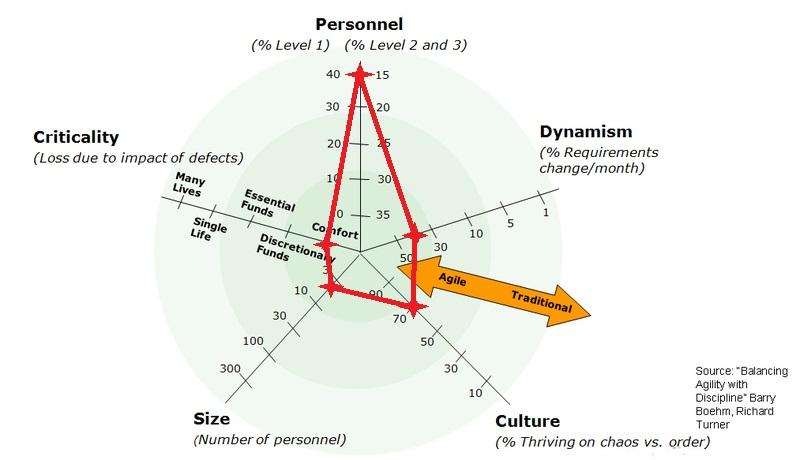
\includegraphics[height=8cm, width=15cm]{RadarChartPaint.jpg}
\end{center}

\noindent\textbf{Personnel:} 40\%

Ud fra antagelsen om at level 1 opnås med 1-2 års erhvervserfaring kan vi ikke placere vores gruppe på dette parameter, men det vi kan gøre i stedet er, at antage at der ikke kun er tale om erhvervserfaring men at “studieerfaring" også er godtaget. På den måde opnår hele vores gruppe level 1 i erfaring, eftersom vi har arbejdet med webudvikling i omtrent et år nu.

\newpage
\noindent\textbf{Dynamism:} 40\%

I den overordnede opgavebeskrivelse blev vi introduceret til dette krav: Additional detailed (weekly) requirements could be given by your product owners. Dette er med til at trække os imod origo. Yderligere med brugen af scrum og XP som udviklingsmetoder samt agil udvikling som vores udviklingsmodel, kan vi vægte kravændringer endnu højere. Krav til vores udvikling kan nemlig ændre sig efter hvert sprint.

\noindent\textbf{Culture:} 70\%

Hvis vi ser på os som udviklerteam, ligger vi højt på dette parameter. Da vi antager dette er en skoleopgave som skal afspejle en rigtig måde at systemudvikle på, må vi placere os mere imod origo end periferien. Grundlaget for dette er, at vi stadig er under uddannelse og lærer at tilpasse os selv og vores udvikling til den nye opnåede viden, vi får serveret. Derfor er det helt essentielt for os som udviklingsteam, at vi kan arbejde i et forandringsmiljø. Det skal dog hertil fremhæves at vi ikke kun kan arbejde i det rene kaos, som godt kan forekomme af de forandringer vi oplever, men faktisk også kan arbejde efter orden og tradition, på baggrund af det vi har lært og de erfaringer, vi har gjort os  hidtil.

\noindent\textbf{Team Size:} 5

Vi er et udviklerteam på 5 medlemmer.

\noindent\textbf{Comfort:} Comfort

Da der er tale om almen webudvikling med ingen effekt på nogle andre end os selv, så kan vi roligt antage at det ikke berører hverken vores økonomi, midler eller menneskeliv generelt, hvis vores test af produktet fejler. Hvis vi derimod skulle lave dette for en aktuel virksomhed, kunne det berøre den pågældende virksomheds økonomi, hvis vores test fejlede i form af at virksomhedens økonomi kan være på spil, hvis softwaren ikke var salgsmæssigt klart til tiden.

\chapter*{8. Konklusion}
\addcontentsline{toc}{chapter}{8. Konklusion}

Det kan udledes gennem hele projektets forløb, at brugen af de agile udviklingsmetoder Scrum og XP skaber et bedre overblik og dermed en lettere fremgang. Vi har tacklet diverse udfordringer, som fx i første sprint, hvor hverken Scrum-meetings eller enkelte XP-praktikker blev brugt, hvilket resulterede i at PO havde kritik. Den øgede indsats i både Scrum og XP blev belønnet med overskud og mere effektiv brug af tid. Ved slutningen af sprint 2 befandt vi i gruppen os i en mere fordelagtig position, og det blev yderligere bekræftet af PO, som ikke kom med yderligere kritik.
Planlægningsfasen af projektet konkluderes at vægte højere end først antaget; fasen har en prominent betydning for det fremtidige arbejde og bør ikke negligeres. Ligeledes skal planlægningen opretholdes, hvilket i dette projekt blev fuldført ved daglige Scrum-møder, der hjalp gruppen med at holde overblikket gennem processen.
Det var ikke optimalt at undlade, at diskutere brugen af XP-praktikker, selvom en stor del på forhånd var indforstået. At have en klar defineret plan for brug, og brugen heraf, må konkluderes at have væsentlig betydning for at sikre, at det fælles mål forbliver synkront blandt alle gruppens medlemmer.
Vi kan  også konkludere, at agil udvikling passede godt til gruppen og at det var en god udviklingsmetode, da processen under projektet forløb godt, efter udviklingsmetoderne blev sat helt på plads. Dog kunne selve planlægningsprocessen godt have været bedre, eftersom der var ting, vi ikke havde tænkt over før vi startede udviklingen af produktet, og som vi endte med at gøre undervejs i stedet. 
Derudover er vores opnåede erfaring med outsourcing helt klart anvendeligt i fremtiden, da vi fik et godt indblik i hvad det vil sige at outsource, samt forholde os kritisk til hvem vi outsourcer hos.

\chapter*{9. Bilag}
\addcontentsline{toc}{chapter}{9. Bilag}

\section*{9.1 Bilag 1) Fully dressed use case}
\addcontentsline{toc}{section}{9.1 Bilag 1) Fully dressed use case }
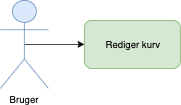
\includegraphics[width=8cm, height=5cm]{FullyDressedUseCase.png}

\noindent \textbf{Use case:} rediger kurv

\noindent \textbf{Primary Actor:} Bruger

\noindent \textbf{Goal:} At redigere produkter i brugerens kurv. 

\noindent \textbf{Scope:} Et produkt salgssystem. Baseret udelukkende på software salg, med en anbefaling til hvilken computer kunne tilkøbes til det software der bliver vist.

\noindent \textbf{Level:} ! (user goal) 

\noindent \textbf{interests:}
\begin{itemize}[topsep=0pt, partopsep=0pt]
  \item[--] Bruger, som gerne vil ændre antallet af et specifikt produkt i kurven.
  \item[--] Bruger, som gerne vil slette et produkt i kurven. 
\end{itemize}

\noindent \textbf{Preconditions:}
\begin{itemize}[topsep=0pt, partopsep=0pt]
  \item[--] Der skal være mindst et produkt i kurven.
\end{itemize}

\newpage
\noindent \textbf{Success Guarantees: }
\begin{itemize}[topsep=0pt, partopsep=0pt]
  \item[--] Databasen er oppe med alle produkterne, således at der kan tilføjes til kurven.
\end{itemize}

\noindent \textbf{Triggers:}
\begin{itemize}[topsep=0pt, partopsep=0pt]
  \item[--] Bruger trykker på slet produkt.
  \item[--] Bruger tilføjer eller fjerne antallet af produkter.
\end{itemize}

\noindent \textbf{Triggers:}
\begin{enumerate}[topsep=0pt, partopsep=0pt]
  \item Brugeren har to produkter i kurven.
  \item Brugeren tilføjer til mængden af et produkt x antal gange.
  \item Brugeren fjerner det andet produkt.
\end{enumerate}


\newpage
\section*{9.2 Bilag 2) Prototype af webdesign}
\addcontentsline{toc}{section}{9.2 Bilag 2) Prototype af webdesign}

\noindent Seeking HTML/CSS designer.

\noindent We are looking for a designer to develop a frontend design for our software web-shop. We have made a sketch/prototype, that you should take inspiration from. We would like the design to contain different buttons, labels and input fields, as seen on the sketch. The designs of the pages are completely up to you. You are allowed the freedom to make your own decisions regarding the looks of the components (e.g. labels, filters, menu bars, etc.).

\noindent The sketch is merely meant as an inspiration. We would however like to emphasize that the design should resemble the fact that we are selling software.

\noindent In the sketches you will see different boxes with P’s in them; these are products. They are meant to be images of said product and the price should be featured somewhere on or close to the product.

\noindent The logo should be a button.

\noindent We would like the filter to feature check boxes, a slider and drop down boxes, all should be reusable.

\noindent Lastly it is only the design and styling you will be responsible for. We will make all functionality and make it compatible with our API.

\noindent On a side note we would much appreciate it if you will feature descriptive comments on your code, as it will be easier to integrate your work with ours.

\noindent \textbf{Header:}\\
\noindent Will contain a logo which has a link to the front page, alongside with a navigation menu with links to subpages, and an icon of a shopping cart which navigates to the shopping cart. 

\noindent \textbf{Footer:}\\
\noindent Has 3 columns:
\begin{enumerate}[topsep=0pt, partopsep=0pt]
  \item Contact information text.
  \item Logo along with copyright information.
  \item Other info about the company or page.
\end{enumerate}

\begin{center}
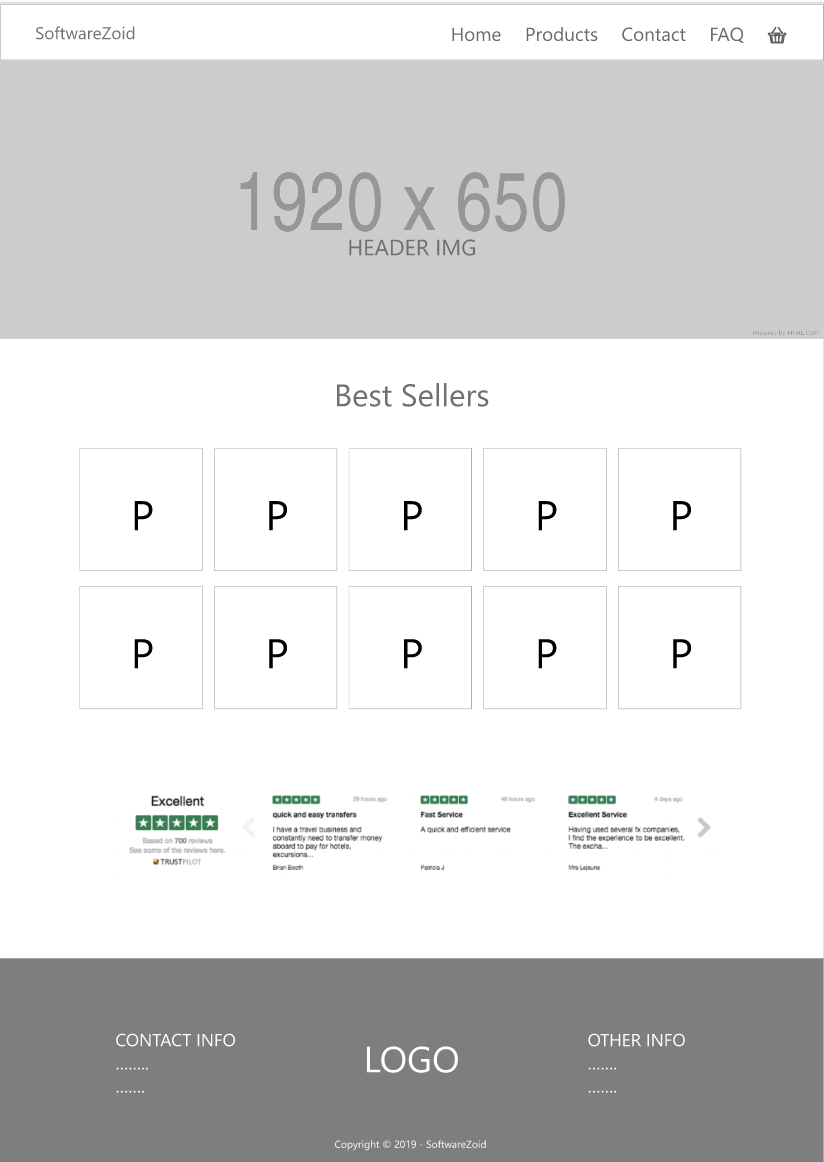
\includegraphics[height=17cm]{page1}
\end{center}
\noindent This page consists of 3 sections:
\begin{itemize}[topsep=0pt, partopsep=0pt]
  \item Header image: The width scales with the page, the height is fixed, though it doesn’t have to be “650”
  \item Best Sellers: Shows the best selling products, where P is the product with an image, title and price.
  \item Reviews: Must show 4 reviews per page in the slider. Contains stars, title, info and name.
\end{itemize}

\begin{center}
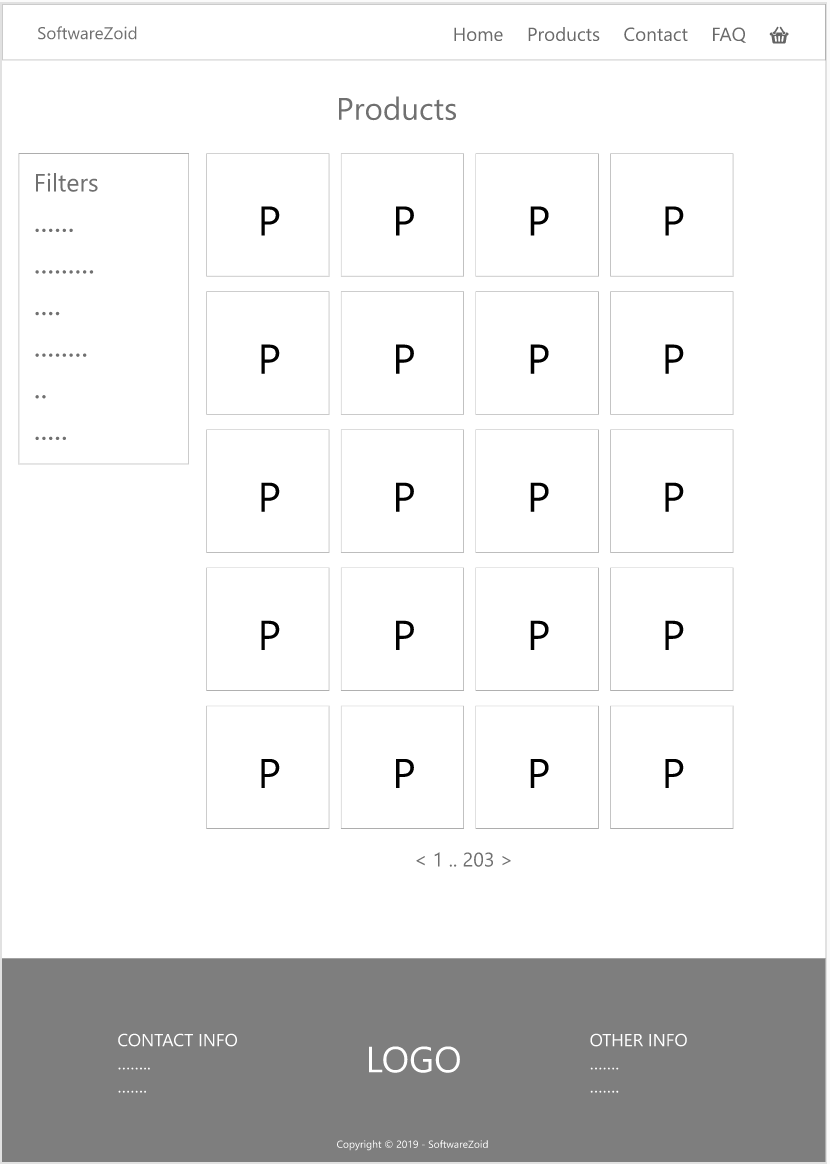
\includegraphics[height=17cm]{page2}
\end{center}
\noindent The products page, for each P(product) it should include an image, title and price. The filters (on the left side) includes a checkbox, slighter and a dropdownbox. The 3 components must be reusable. We also need pagination under each product.

\begin{center}
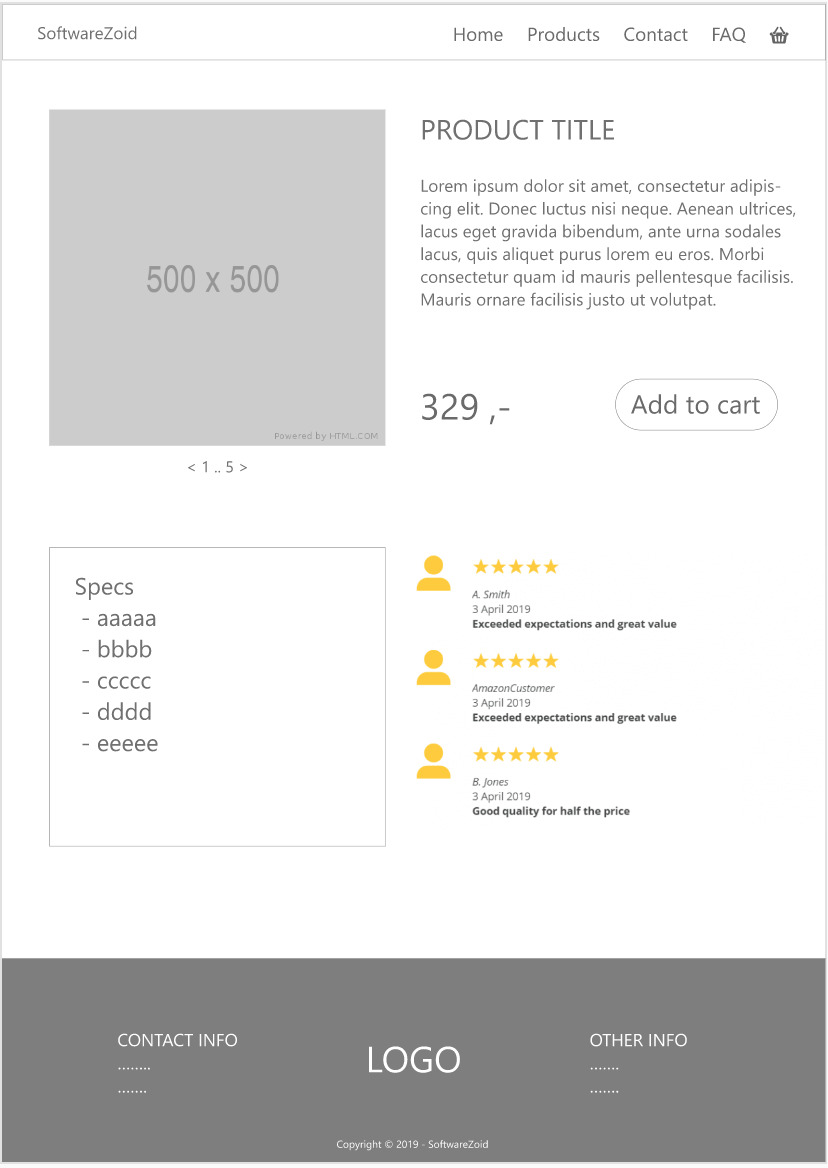
\includegraphics[height=17cm]{page3}
\end{center}
\noindent This page consists of images of the given product with pagination under it. The page includes a product title, a description of the product and a button. The specs must be made as a table of the most important information on the product. This page also includes reviews of the product which includes a rating, name, date and info.

\begin{center}
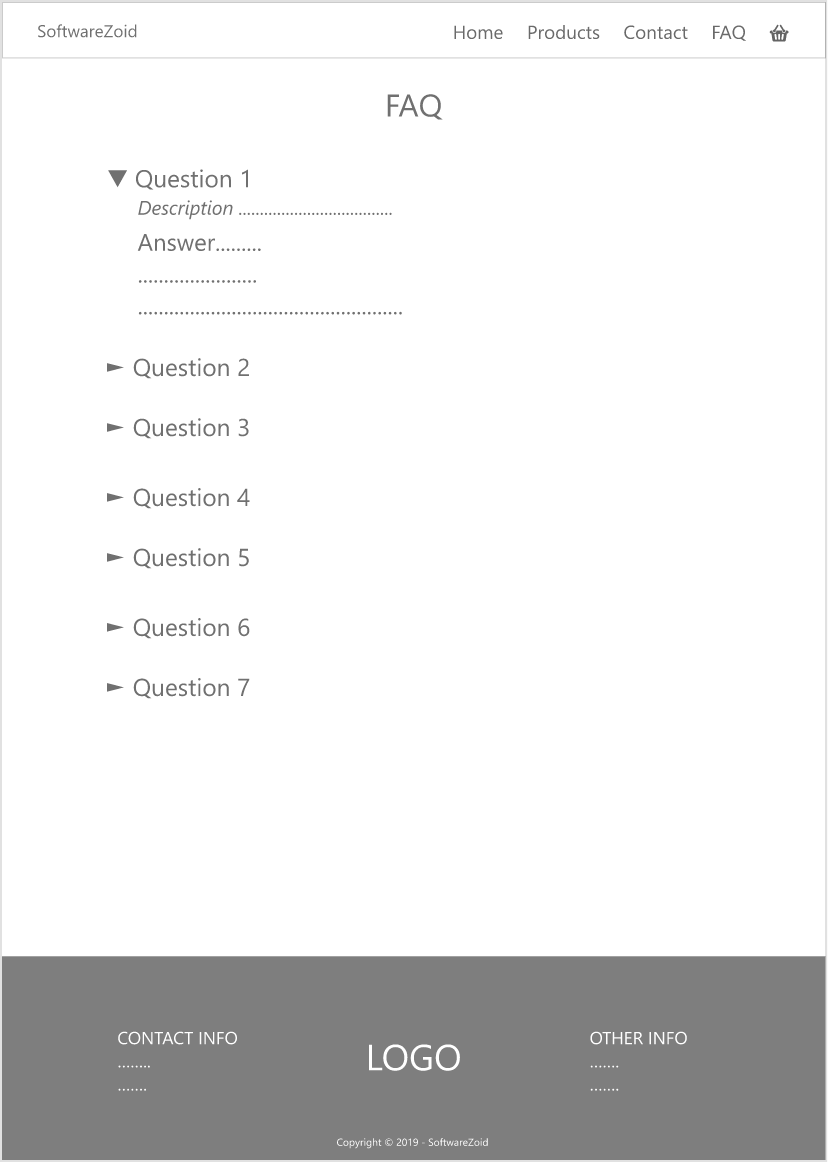
\includegraphics[height=17cm]{page4}
\end{center}
\noindent FAQ has 1 section
\begin{itemize}
  \item This section consists of several questions of which are dropdowns. The description and answer to the question is only shown when the question is clicked/opened.
\end{itemize}

\begin{center}
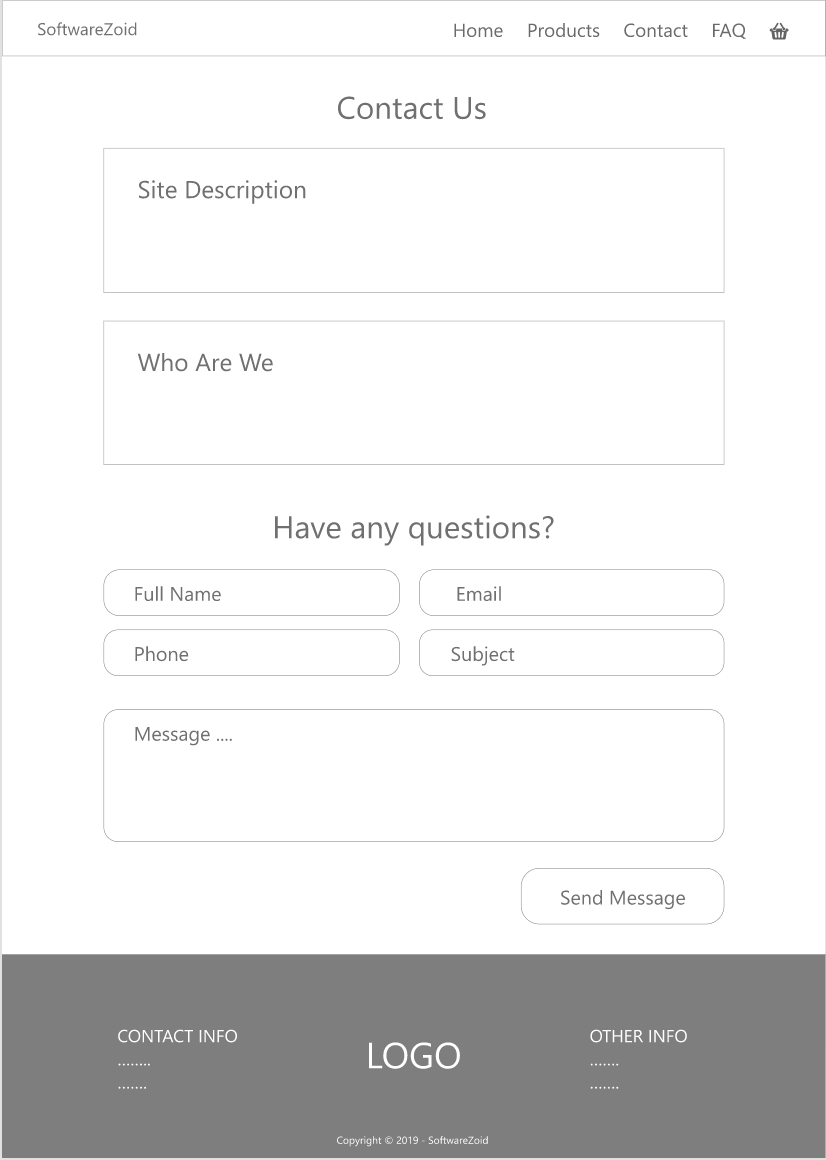
\includegraphics[height=17cm]{page5}
\end{center}
\noindent The contact page consist of 3 sections:
\begin{itemize}
  \item A site description and a “who are we”: Has to show a lot of text in a pretty and manageable way.
  \item Have any Questions: a form with these input fields: full name, email, phone, subject and message.
\end{itemize}

\begin{center}
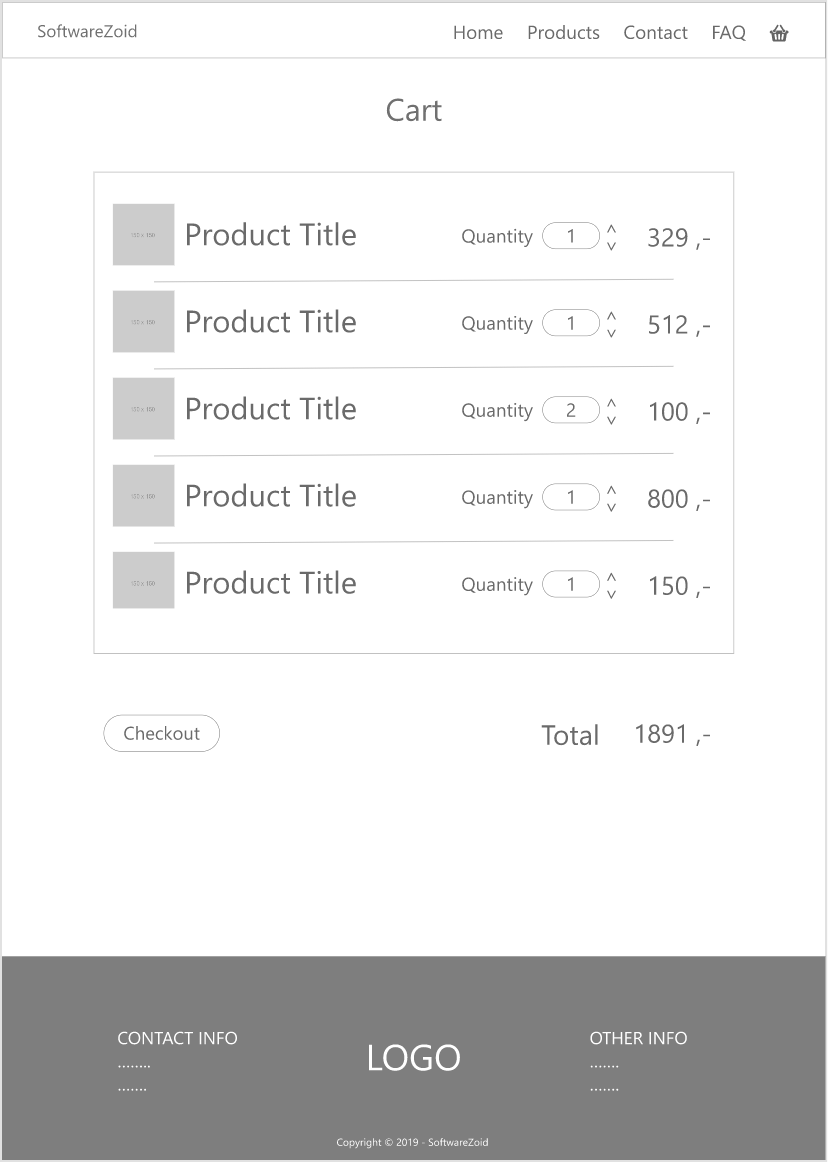
\includegraphics[height=17cm]{page6}
\end{center}
\noindent The cart page has a list of all the products that the customer has put in their basket, has to be presented in a table. In each table row there must be a product image, a product title, a display of quantity, and a price. Under the table there has to be a checkout button, alongside with a total price for all products in the basket.

\begin{center}
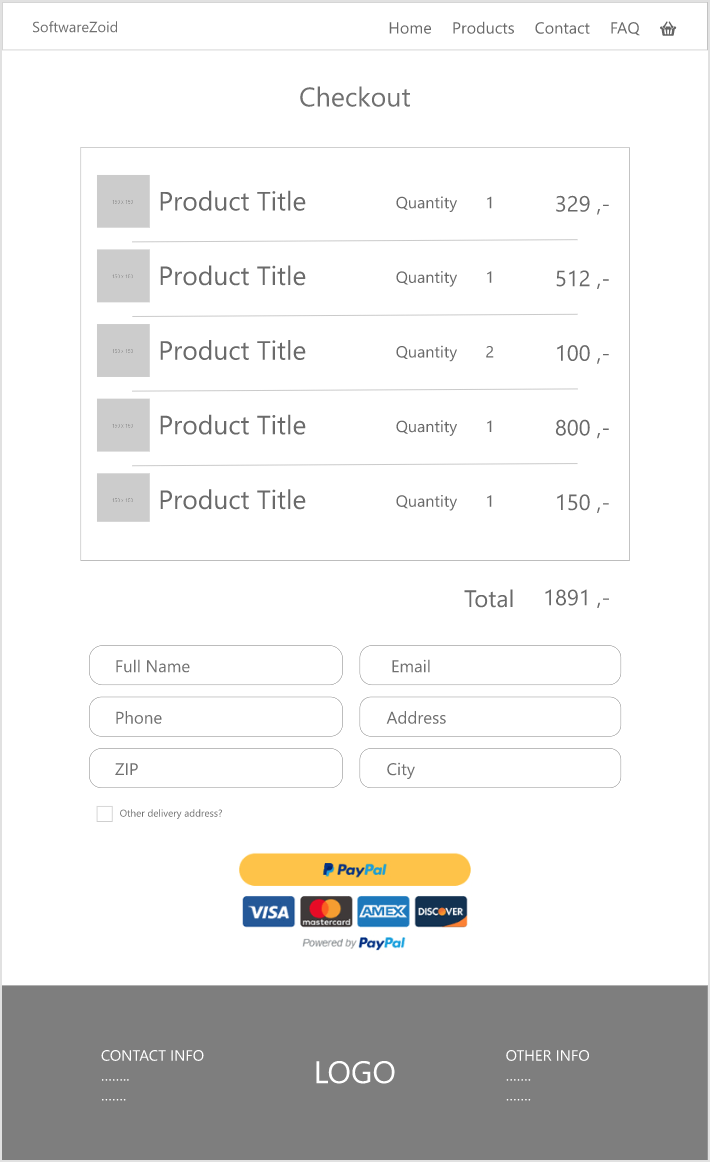
\includegraphics[height=17cm]{page7}
\end{center}
\noindent The checkout page will contain a list of the products that were put in cart, shown in a table. In each table row there has to be a product image, product title, quantity and product price. Under the table there has to be a display of the total price and a checkout form. The checkout form must contain following fields: full name, email, phone, address, zip and city, the form must also include a checkbox for alternative shipping address. Lastly a pay with paypal button.

\newpage
\section*{9.3 Bilag 3) Outsorce Korrespondance af webdesign}
\addcontentsline{toc}{section}{9.3 Bilag 3) Outsorce Korrespondance af webdesign}

\noindent\underline{Tuesday, November 12, 2019 – Andreas Vikke}\\
\noindent We're a team of backend developers that are working with a client that sells software and software packages.

\noindent We're looking for a frontend designer with a simplistic form of creativity, and likes the creative style of minimalism. The actual design of the frontend page(s) is not specified, you will be provided a sketch of how and where labels and buttons should be places, but we will gladly take input from you if you have better ideas.

\noindent We do although require that the code is documented to some degree with comments so that we can more smoothly integrate it with our backend. We also require that you as the designer can both understand, and write English.

\noindent The sketch is made in Adobe XD, and provided here there's a demo page:

\noindent https://xd.adobe.com/view/5da95fa7-c677-44d6-6430-3383f6cf8c37-2b98/ (Bilag 2)

\noindent (Attached is the 3 files: The Sketch in PDF and XD format, and a general description PDF of all the pages)

Est. Budget: \$200.00

Milestone 1: Basic Structure / design

Due: Friday, November 15, 2019

Amount in escrow: \$50.00 

\noindent\underline{Tuesday, November 12, 2019 – Andreas Vikke}\\
\noindent Hello Ahmed, I found your profile and previous work very well done, and I'm hoping you'll accept our offer. If you have any questions regarding the milestones or their meanings please do contact me.

\noindent\underline{Tuesday, November 12, 2019 – Ahmed Hassan}\\
\noindent Hello Andreas I will check the attached files now and get back to you

\noindent\underline{Tuesday, November 12, 2019 – Andreas Vikke}\\
\noindent Perfect, thank you.


\noindent\underline{Tuesday, November 12, 2019 – Ahmed Hassan}\\
\noindent Hello Andreas, I checked the files and I can start in anytime , thank you.

\noindent\underline{Tuesday, November 12, 2019 – Ahmed Hassan}\\
\noindent Ahmed Hassan accepted the offer

\noindent I will start now can I know if you use angular for front-end ?

\noindent also I will use scss is this good for you or you preferred css ?

\noindent\underline{Tuesday, November 12, 2019 – Andreas Vikke}\\
\noindent We use react for front end, not angular.

\noindent You can use scss, as long as you provide us with a css file afterwards

\noindent Both the scss and css file i mean :)

\noindent\underline{Tuesday, November 12, 2019 – Ahmed Hassan}\\
\noindent great, thank you.

\noindent\underline{Tuesday, November 12, 2019 – Andreas Vikke}\\
\noindent Looking forward to seeing what you make :)

\noindent\underline{Tuesday, November 12, 2019 – Ahmed Hassan}\\
\noindent I will do my best :)

\noindent\underline{Tuesday, November 14, 2019 – Andreas Vikke}\\
\noindent Hello Ahmed, do you have some basic structure and design you can show me as per the first milestone? :)

\noindent\underline{Tuesday, November 14, 2019 – Ahmed Hassan}\\
\noindent Hello Andreas, I will give you tonight the layout and home page, don’t worry :)


\noindent\underline{Tuesday, November 15, 2019 – Ahmed Hassan}\\
\noindent Ahmed Hassan requested payment for the milestone

\noindent this is the layout and home page also I create a global css buttons and selectors.

\noindent I added overview section, our team and contact us.I think Contact us is important to be in home page but if you want to delete any section I will.

\noindent please give me your feedback or changes If you want to change anything

Milestone 1: "Basic Structure / design"

Due: Friday, November 15, 2019

Amount: \$50.00

\noindent\underline{Tuesday, November 15, 2019 – Andreas Vikke}\\
\noindent Hello Ahmed, at first glance it looks great! my team is just reviewing it and coming with thoughts and changes, then i will send them and the money to you :)

\noindent\underline{Tuesday, November 15, 2019 – Ahmed Hassan}\\
\noindent Okay and also I will update small things to improve the homepage :)

\noindent\underline{Tuesday, November 15, 2019 – Andreas Vikke}\\
\noindent Sounds great! :)

\noindent\underline{Tuesday, November 15, 2019 – Andreas Vikke}\\
\noindent Hello Ahmed, everything seems very well. It seems like the buttons aren't really going to the right places though, FAQ goes to "best sellers", basket goes to contact us, contact us goes to a "about us" section. I'm assuming this is because the faq and cart page haven't been made yet? :)

\noindent We like the OPA style that you've made, although we don't need an about us section as a "our team" sort of thing.

\noindent I think it's a good idea with the contact section being on the home page, i haven't heard any comments from my team regarding this though, so we'll keep it like that for now :)

\noindent Now that the basic structure and design is in place, we're just missing some of the remaining pages (Specifik product page, FAQ, basket and checkout). As said you still have your artistic freedom over these pages as long as long as it has the requirements from the sketch (e.g. specific product has title, description, price and so on).

\noindent If you have any questions or uncertainties, don't hesitate to write me, I'll respond as quickly as possible.

\noindent Looking forward to what you produce :)

\noindent Andreas Vikke approved the milestone

Milestone 1: "Basic Structure / design"

Due: Friday, November 15, 2019

Amount paid: \$50.00

Amount: \$50.00

\noindent Andreas Vikke activated the milestone

Milestone 2: "Final Outcast/Evaluation"

Due: Sunday, November 17, 2019

Amount: \$50.00

\noindent\underline{Tuesday, November 15, 2019 – Andreas Vikke}\\
\noindent For the final Outcast we'd like that the specific single products get their own page, as well as faq, basket and checkout. :)

\noindent\underline{Tuesday, November 16, 2019 – Ahmed Hassan}\\
\noindent Don’t worry in the final outcast everything will be like you want :)

\noindent\underline{Tuesday, November 16, 2019 – Andreas Vikke}\\
\noindent Perfect! :)
\newpage
\noindent\underline{Tuesday, November 16, 2019 – Ahmed Hassan}\\
\noindent Ahmed Hassan requested payment for the milestone

\noindent please check the whole website design and I still have some work with it

Milestone 2: "Final Outcast/Evaluation"

Due: Sunday, November 17, 2019

Amount: \$50.00

\noindent\underline{Tuesday, November 16, 2019 – Andreas Vikke}\\
\noindent Hello Ahmed, very impressive! :)

\noindent We do have a few pointers though:

\noindent I can see you haven't quite finished the contact page, and that the navlink contact currently goes to whatever page it is currently on, that of course just needs fixing and I'm assuming that this is what you mean with you still have some work to do :)

\noindent On the basket page i can see that there's a payment option, we only want that in the checkout page.

\noindent On the product page, the filter tab is responsive with the body and the body shrinks according to the filter, but the footer does not, we'd like that it does as well.

\noindent I can see we are also missing the page when you click on "more details" on a product. i can see it's there, it's just not linked from what i can get. :)

\noindent I haven't been able to check yet wether or not it looks nice on mobile, but this is also important to us, that the website can adapt to this.

\noindent So just the last bits and mobile friendly and we're about there! We're very happy with what you've provided so far, looks very nice!

\noindent Andreas Vikke approved the milestone

Milestone 2: "Final Outcast/Evaluation"

Due: Sunday, November 17, 2019

Amount paid: \$50.00

Amount: \$50.00
\newpage
\noindent Andreas Vikke activated the milestone

Milestone 3: "Final Product"

Due: Tuesday, November 19, 2019

Amount: \$100.00


\noindent\underline{Tuesday, November 19, 2019 – Andreas Vikke}\\
\noindent Did you see and understand my message Ahmed? :)

\noindent\underline{Tuesday, November 19, 2019 – Ahmed Hassan}\\
\noindent Yes I am working now to give you final design :)

\noindent\underline{Tuesday, November 19, 2019 – Andreas Vikke}\\
\noindent Perfect! :)

\noindent\underline{Tuesday, November 19, 2019 – Ahmed Hassan}\\
\noindent Ahmed Hassan requested payment for the milestone

\noindent Milestone 3: "Final Product"

Due: Tuesday, November 19, 2019

Amount: \$100.00    

\noindent this the final version please check it and if you face any problem send to me anytime also if you face any problem in my work after closing the contract I will fix it for free :)


\noindent\underline{Tuesday, November 19, 2019 – Andreas Vikke}\\
\noindent Perfect, we're just going to look it through and I'll come back to you, at first glance here it looks amazing :)

\noindent\underline{Tuesday, November 19, 2019 – Andreas Vikke}\\
\noindent I've sent it off to the rest of my team, and awaiting to hear some response and feedback from them, but i noticed some small details I'd liked fixed :)

\noindent When in basket, continue shopping doesn't go to products.

\noindent Also in basket, the home link doesn't respond when clicked (can't go from basket to home).

\noindent When on products page, notice how it's not the same logo in the cart as in all other pages, we'd like that the logo for the cart is consistent throughout the pages.

\noindent That's what i just noticed quickly looking through it, I'll send the feedback if i get any later today, and if i don't get anything I'll just send you the money :)

\noindent\underline{Tuesday, November 19, 2019 – Ahmed Hassan}\\
\noindent okay bro, I fixed the issues that you noticed :)

\noindent\underline{Tuesday, November 19, 2019 – Andreas Vikke}\\
\noindent It looks good, some things went missing and/or misaligned though

\noindent Filter icon gone and misalignments in the cart

\noindent\underline{Tuesday, November 19, 2019 – Ahmed Hassan}\\
\noindent oh, sorry :D

\noindent\underline{Tuesday, November 19, 2019 – Andreas Vikke}\\
\noindent Perfect, thanks ^^ haven't heard back from my team yet, but expecting some feedback soon! :)

\noindent\underline{Tuesday, November 19, 2019 – Andreas Vikke}\\
\noindent So what seems to be the last feedback is that we'd like a "back" button from product details to products, do you think you could do that quickly? :)

\noindent\underline{Tuesday, November 19, 2019 – Ahmed Hassan}\\
\noindent I added it :)

\noindent\underline{Tuesday, November 19, 2019 – Andreas Vikke}\\
\noindent Perfect, thank you very much ^^ My team doesn't seem to have any more feedback, so i thank you for your help! :)

\noindent Andreas Vikke approved the milestone

Milestone 3: "Final Product"

Due: Tuesday, November 19, 2019

Amount paid: \$100.00

Amount: \$100.00

\noindent\underline{Tuesday, November 19, 2019 – Andreas Vikke}\\
\noindent Andreas Vikke ended the contract

\noindent\underline{Tuesday, November 19, 2019 – Ahmed Hassan}\\
\noindent thanks you very much , I am here anytime if you need any help :) I hope you give me a good feedback :)

\noindent\underline{Tuesday, November 19, 2019 – Andreas Vikke}\\
\noindent Thank you very much :) and I've given you 5 stars a long with a good review text :D

\noindent\underline{Tuesday, November 19, 2019 – Ahmed Hassan}\\
\noindent thank you :)


\newpage
\section*{9.4 Bilag 4) Outsorce Korrespondance af 404 side}
\addcontentsline{toc}{section}{9.4 Bilag 4) Outsorce Korrespondance af 404 side}

\noindent\underline{3. Dec. - William Huusfeldt}
\begin{enumerate}
\item \textbf{Your existing website link to get the feel of your website.}
The website that we're building is linked below.
softwarezoid.surge.sh
\item \textbf{Any special requirements for your design}
Be as creative as you like, however, we'd like it that the page reflects that we're dealing with software sales.
\end{enumerate}

\noindent\underline{3. Dec. - Mizanur}\\
\noindent Hello, thanks very much for your order. Unfortunately, I am out of my workplace until tomorrow. Will it be possible for you to increase the deadline by 2 days? I promise to get back to work as soon as I return to my workplace. Thanks.

\noindent\underline{3. Dec. - William}\\
\noindent Hi again, That's quite alright.

\noindent\underline{3. Dec. - Mizanur}\\
\noindent Thank you very much. I really appreciate it.

\noindent\underline{3. Dec. - Mizanur}\\
\noindent to clarify, you need a 404 page design both in Photoshop and HTML and CSS? 
\noindent Did I get it right?

\noindent\underline{3. Dec. - William}\\
\noindent No problem :)
\noindent HTML and CSS is top priority and actually mainly what we're looking for, and yes, it's a 404 page we'd like to get.

\noindent\underline{3. Dec. - Mizanur}\\
\noindent Thank you for your reply. I will get back to you as soon as I can. In the meantime, I am sending you a request to extend the deadline by two days. Please accept. Thanks.

\noindent -- Deadline rykkes 2 dage til d. 7. Dec.

\noindent\underline{6. Dec. - Mizanur}\\
\noindent Hello, I have made designed the page. I have followed the design style, color and font combination of your current website. I hope you will like it. Please have a look and give your feedback. Thanks.

\noindent\underline{6. Dec. - William}\\
\noindent Perfect, thank you!

\noindent\underline{6. Dec. - Mizanur}\\
\noindent Hi willhuusfeldt,
\noindent Thanks again for your order! Your delivery is enclosed. You will find the source files in the zip format attached here. If there are any problems, please let me know. I'll get back to you as soon as I can.

\noindent If you need anything to change in the design please message me. Don't forget to appreciate me in the comments.

\noindent Thanks again and have a great day! :)

\noindent Mdmizanur3950

\noindent -- Godkendt


\newpage
\section*{9.5 Bilag 5) Outsorce Korrespondance af Favicon}
\addcontentsline{toc}{section}{9.5 Bilag 5) Outsorce Korrespondance af Favicon}


\noindent\underline{4. Dec. - William Huusfeldt:}\\
\noindent This is our website softwarezoid.surge.sh

\noindent We don't have a logo per se, so take inspiration from the site and make something that you think fits the site.

\noindent Regards, William

\noindent\underline{4. Dec. - Pro\_Graphics\_4U:}\\
\noindent Hey willhuusfeldt, please see the attached files.

\noindent I added you even bonus (source file)

\noindent Before leaving feedback, please let me know if you have ANY issues with your files and I'll do everything in my power to correct it for you at no additional charge.

\noindent If you like it, I would sincerely appreciate a good and honest review.

\noindent I want you to be 100\% satisfied with my work, otherwise, I insist that you ask me for a full refund. No hard feelings.

\noindent Ps. Do you have any more work to do? Or something you are struggling with?

\noindent Thank you, Regards Cris

\noindent -- Godkendt


\newpage
\section*{9.6 Bilag 6) Retrospective Meetings}
\addcontentsline{toc}{section}{9.6 Bilag 6) Retrospective Meetings}
\noindent\textbf{Retrospektiv møde - Spint 1, Fredag d. 22/11}\\
\noindent Gruppen som helhed, mente der var positiv feedback. Sprintets udvalgte user stories var alle på nær en enkelt blevet færdigudviklet, men holdes “åbne” for eventuelle fremtidige modificeringer. Internt i gruppen er der blevet reflekteret over det første sprint. Her er stemningen, at arbejdsfordelingen har været velfungerende og passende, hvorfor det også menes at første sprint har været effektivt; vi har udviklet meget og sat os i en fin position i forhold til de fremtidige sprint. Det menes også at selvstændigheden har fremmet det positive arbejde. Dog ønsker vi i gruppen at øge indsatsen for pair programming til næste sprint, så vi forhåbentlig kan udbedre nogle af de kommunikationsproblemer, der har præget arbejdet i dette sprint. Ydermere var den eneste konklusion at drage vedr. Estimering af tid på user stories: dette skal forbedres. Estimeringerne var konsekvent forkerte. På baggrund af det har vi diskuteret og ændret estimeringer på alle andre user stories, for at imødekomme fejlene og forhåbentlig give en mere præcis estimering.

\noindent\textbf{Retrospektiv møde - Spint 2, Mandag d. 2/1}\\
\noindent Godt med pair programming - fungerede godt på zoom. Det var både effektivt og hyggeligt. De velfungerende elementer fra sidste sprint er blevet taget med videre til dette. Ydermere har vi taget kritikken fra sidste sprint og forsøgt at udbedre disse, hovedsageligt har gruppen fokuseret på at inkorporere pair programming mere, hvilket var et ønske blandt medlemmerne fra sidst. Arbejdet var effektivt, men en user story i dette sprint blev ikke udviklet -- arbejdet blev ikke påbegyndt. Dette er på baggrund af, at datasættet vi skulle bruge, ikke var blevet leveret i en tilstand, hvor gruppen kunne arbejde på det hvor der var tilstrækkelig tid til det. Arbejdsfordelingen har fortsat været god og fungeret godt med pair programming. Der er kommet øget ønske blandt medlemmerne på at påbegynde dokumentationen, rapporten.

\noindent\textbf{Retrospektiv møde - Spint 3, Fredag d. 6/1}\\
\noindent Der var fin tilfredshed i gruppen over, at arbejdet på projektet har været så langt henne, så der kunne fokuseres på de sidste detaljer. De velfungerende aspekter fra sidste sprint var blevet taget med i dette, dog mener nogle medlemmer, er deres egen arbejdsindsats ikke har været på et tilstrækkeligt niveau. I sprintet blev vi også udsat for en mindre ubekvemhed; gruppen vi arbejder sammen havde undladt at informere os om, at de havde gået væk fra deres oprindelige idé om at sælge hardware. Et ønske fra flere medlemmer var at bruge tid på rapporten, som fik muligheden grundet den relativt lille mængde programmering som manglede. Alle user stories blev lavet færdig og en unødvendig blev skrottet, eftersom denne ikke ville give mening at lave.

\newpage
\section*{9.7 Bilag 7) User stories}
\addcontentsline{toc}{section}{9.7 Bilag 7) User stories}
\noindent\textbf{Sprint-1}

\noindent\textbf{\#1 Som bruger vil jeg gerne kunne se en liste af software.}\\
\noindent En bruger skal kunne se en liste af softwares, hvor de herefter kan klikke ind og få mere information omkring det enkelte software.
\noindent Acceptens krav:
\begin{itemize}[topsep=0pt, partopsep=0pt]
  \item Alle produkter skal have billede, titel og pris.
  \item Billeder, titel og pris skal hænge sammen med produktet.
  \item Listevisning skal fremvises på en præsentabel måde.
\end{itemize}
\noindent Subtasks:
\begin{itemize}[topsep=0pt, partopsep=0pt]
  \item \#14 Sidens liste skal kunne vise en titel for hvert software.
  \item \#15 Sidens liste skal kunne vise pris for hvert software.
  \item \#16 Sidens liste skal kunne vise en thumbnail.
  \item \#89 Listen skal bruge en DTO klasse til fremvisning af en software givet fra databasen (Titel, thumbnail, description).
  \item \#90 Listen skal hente software gennem et rest-endpoint, som returnere en DTO klasse.
  \item \#91 Opret en entitet til software, med de forskellige fields der skal gemmes i database. (Titel, thumbnail, description).
  \item \#92 Opret facade som fetcher software fra databasen og omdanner den til DTO’en.
\end{itemize}

\noindent\textbf{\#17 Som bruger vil jeg gerne kunne se information om et enkelt software.}\\
\noindent Som bruger vil jeg gerne have at jeg kan tilgå softwares fra en database, således at de tilgængelige software hele tiden er opdateret.
\noindent Acceptens krav:
\begin{itemize}[topsep=0pt, partopsep=0pt]
  \item Informationen om softwaren skal kunne vises på en hjemmeside.
  \item Hvert software skal være på hver sin side.
\end{itemize}
\noindent Subtasks:
\begin{itemize}[topsep=0pt, partopsep=0pt]
  \item \#93 Siden skal kunne vise en titel for hvert software.
  \item \#95 Siden skal kunne vise pris for hvert software.
  \item \#97 Siden skal kunne vise en thumbnail.
  \item \#98 Siden skal kunne vise en description.
  \item \#99 Listen skal hente software gennem et rest-endpoint, som returnere en DTO klasse(getSingle).
  \item \#100 Opret facade som fetcher software fra databasen og omdanner den til DTO’en(getSingle).
  \item \#112 Siden skal kunne vise specifikationer.
\end{itemize}

\noindent\textbf{\#4 Som bruger vil jeg gerne kunne se et softwares indhold ved at navigere gennem listen.}\\
\noindent Der skal kunne fremvises en liste af softwares, hvor der kan fremvises detaljer om hvert software.
\noindent Acceptens krav:
\begin{itemize}[topsep=0pt, partopsep=0pt]
  \item Der skal kunne være en knap der navigere til det valgte produkt.
  \item Der skal være en knap fra produktsiden der navigerer tilbage til listen over produkter.
  \item Sammenhæng mellem produkt og liste.
\end{itemize}
\noindent Subtasks:
\begin{itemize}[topsep=0pt, partopsep=0pt]
  \item \#94 Opret links til softwaren.
  \item \#96 Opret routing til softwaren.
\end{itemize}

\noindent\textbf{\#64 Som bruger vil jeg kunne se ofte stillede spørgsmål.}\\
\noindent En FAQ side, som beskrevet er ofte stillede spørgsmål med deres besvarelser.
\noindent Acceptens krav:
\begin{itemize}[topsep=0pt, partopsep=0pt]
  \item Skal være relevante spørgsmål ift. brugeren.
  \item Svaret skal hænge sammen med spørgsmålet.
  \item Spørgsmålene skal være enkle.
\end{itemize}
\noindent Subtasks:
\begin{itemize}[topsep=0pt, partopsep=0pt]
  \item \#83 Opret FAQ side.
  \item \#84 Opret liste visning af spørgsmål og svar.
  \item \#85 Skriv spørgsmål og deres tilhørende svar.
\end{itemize}

\noindent\textbf{\#66 Som bruger vil jeg kunne se min indkøbskurv, hvor jeg kan tilføje og fjerne produkter.}\\
\noindent Indkøbskurven har alle de produkter man har valgt. Hertil skal produkter tilføjes, men hvis kunden skifter mening skal kunden kunne slette produktet. Ønsker kunnen flere eller færre af samme produkt, skal kunnen også kunne ændre på dette fra deres indkøbskurv.
\noindent Acceptens krav:
\begin{itemize}[topsep=0pt, partopsep=0pt]
  \item Alle produkter skal gemmes i en session.
  \item Visning af alle produkter skal være overskueligt.
  \item Når et produkt rammer en quantity på 0 skal varen slettes.
  \item Samlet pris skal være korrekt ift. de produkter der er valgt.
  \item Prisen på produkterne skal være samme priser som produkterne viste på produkt siden.
\end{itemize}
\newpage
\noindent Subtasks:
\begin{itemize}[topsep=0pt, partopsep=0pt]
  \item \#74 Vis software i liste fra cookie.
  \item \#76 Tilføj quantity funktion.
  \item \#78 Lav knap til at fjerne software fra liste.
\end{itemize}

\noindent\textbf{\#87 Spike: Læse op på React billede håndtering.}
\begin{itemize}[topsep=0pt, partopsep=0pt]
  \item \#73 Vis en liste a valgte produkter. (Pris, titel og billede). 
  \item \#75 Vis samlet pris for alle software.
  \item \#77 Tilføj knap til checkout.
\end{itemize}

\noindent\textbf{Sprint-2}

\noindent\textbf{\#67 Som bruger vil jeg kunne skrive og se en anmeldelse af et produkt.}\\
\noindent Når en bruger har købt et produkt, skal brugeren have mulighed for at anmelde det, således at andre brugere kan se hvad andre synes om produktet.
\noindent Acceptens krav:
\begin{itemize}[topsep=0pt, partopsep=0pt]
  \item Review skal have en titel og der skal være givet 1-5 stjerner.
  \item Det er valgfrit at komme med en beskrivelse til anmeldelse.
  \item Anmeldelsen skal have en dato på hvornår den var indgivet.
\end{itemize}
\noindent Subtasks:
\begin{itemize}[topsep=0pt, partopsep=0pt]
  \item \#72 Anmeldelsen skal gemmes til produktet og vises på produktet.
\end{itemize}

\noindent\textbf{\#105 Som kunde, vil jeg gerne kunne komme i kontakt med firmaet.}\\
\noindent Som kunde skal jeg kunne kontakte firmaet hvis jeg har et problem eller har spørgsmål til noget.
\noindent Acceptens krav:
\begin{itemize}[topsep=0pt, partopsep=0pt]
  \item En kontakt formular skal kunne oprettes og vises.
  \item Kontakt formularer som er færdigbehandlet skal ikke vises.
\end{itemize}
\noindent Subtasks:
\begin{itemize}[topsep=0pt, partopsep=0pt]
  \item \#106 Siden skal indeholde en formular, således at kunden kan kontaktes (navn, nummer, mail, emne og besked).
  \item \#107 Siden skal indeholde information om kontakten (nummer, lokation, mail).
  \item \#108 Formularen skal gemmes i en databasen.
  \item \#109 Man skal kunne hente alle formularer igennem et rest endpoint.
  \item \#110 Opret facade metode der fetcher formularer og omdanner dem til DTO'er, således at der ikke er dato eller behandlings status.
\end{itemize}

\noindent\textbf{\#116 Som bruger vil jeg gerne kunne filtrere produkt siden.}\\
\noindent Acceptens krav:
\begin{itemize}[topsep=0pt, partopsep=0pt]
  \item Filtrere produkt efter titel.
  \item Filtrere produkt efter pris.
\end{itemize}
\noindent Subtasks:
\begin{itemize}[topsep=0pt, partopsep=0pt]
  \item \#129 Endpoint, getall med en parameter for kategorier.
  \item \#130 Endpoint, der kan get all kategorier.
  \item \#131 Frontend, Filter bar, med kategorier fra databasen.
  \item \#132 Frontend, når en kategori bliver valgt skal den fetche nye produkter.
\end{itemize}

\noindent\textbf{\#115 Som sælger vil jeg gerne se en liste af brugerhenvendelser.}\\
\noindent Acceptens krav:
\begin{itemize}[topsep=0pt, partopsep=0pt]
  \item En liste over brugerhenvendelser
  \item Mulighed for afslutte og slette henvendelser
\end{itemize}
\noindent Subtasks:
\begin{itemize}[topsep=0pt, partopsep=0pt]
  \item \#122 Opret facade som fetcher data fra databasen og omdanner det til DTO.
  \item \#123 Listen skal bruge en DTO klasse til at vise data fra databasen.
  \item \#124 Listen skal hente en DTO klasse gennem et rest-endpoint.
  \item \#125 Listen skal vise titel på henvisning.
  \item \#126 Listen skal vise navn på afsenderen af henvisningen.
  \item \#127 Listen skal vise dato for henvisningen.
  \item \#128 Listen skal vise ID på henvisningen.
\end{itemize}

\noindent\textbf{Sprint-3}

\noindent\textbf{\#34 Som bruger vil jeg gerne kunne se en computer ud fra en anden sides API.}\\
\noindent Acceptens krav:
\begin{itemize}[topsep=0pt, partopsep=0pt]
  \item Skal være på produkt siden.
  \item Skal kunne vise en computer ud fra en fane. 
\end{itemize}
\noindent Subtasks:
\begin{itemize}[topsep=0pt, partopsep=0pt]
  \item \#144 Fetch metode der henter fra eksternt API.
  \item \#145 Liste visning af computer.
  \item \#146 Fane til computeren.
\end{itemize}

\noindent\textbf{\#35 Som sælger vil jeg kunne tilgå en side hvor man kan tilføje software.}\\
\noindent Der skal kunne tilføjes software til databasen gennem webapplikationen, fra en side lavet til dette formål.
\noindent Acceptens krav:
\begin{itemize}[topsep=0pt, partopsep=0pt]
  \item Oprette en side til tilføjelse af software.
  \item Siden skal kunne tage imod alle informationer fra en software som input.
  \item Siden skal kunne tage imod et billede (url f.eks.).
  \item Siden skal have en knap der tilføjer softwaren baseret på input informationen.
\end{itemize}
\noindent Subtasks:
\begin{itemize}[topsep=0pt, partopsep=0pt]
  \item \#133 Nødvendige facade metoder.
  \item \#134 Rest API med POST.
  \item \#135 Javascript der håndtere eventet når man trykker på knappen.
  \item \#136 Javascript der fetcher med POST.
  \item \#137 Tilkobling af javascriptet på HTML.
  \item \#138 Tilføje HTML side.
  \item \#139 Lave tests.
\end{itemize}

\noindent\textbf{\#113 Som bruger vil jeg gerne kunne checke mine varer i indkøbskurven ud og få en faktura.}\\
\noindent Som bruger vil jeg gerne kunne checke de varer, som jeg har tilføjet til indkøbskurven, ud.
\noindent Acceptens krav:
\begin{itemize}[topsep=0pt, partopsep=0pt]
  \item En kunde skal kunne se en liste over valgte produkter (indkøbskurven).
  \item En kunde skal kunne trykke på en knap når de varerne er blevet valgt.
  \item En kunde skal kunne se datoen for købet.
  \item En kunde skal kunne se prisen for købet.
\end{itemize}
\noindent Subtasks:
\begin{itemize}[topsep=0pt, partopsep=0pt]
  \item \#117 Tilføj javascript med fetch til checkout-knappen.
  \item \#118 Oprette entity klasse til en kvittering.
  \item \#119 Oprette REST API til entity klassen.
  \item \#120 Oprette facade klasse til entity klassen med metoder til at kunne gemme og læse entiteter fra databasen.
\end{itemize}

\noindent\textbf{\#121 Som sælger vil jeg gerne se en enkelt brugerhenvendelser ud fra listen.}\\
\noindent Acceptens krav:
\begin{itemize}[topsep=0pt, partopsep=0pt]
  \item Der skal vises en enkelt bruger henvendelse ud fra listeform ved tryk.
  \item En bruger henvendelse skal indeholde navn, dato og description.
\end{itemize}

\noindent\textbf{\#88 Spike: Læse op på Hardware API.}

\end{document}

